\documentclass{article}

\usepackage{geometry}
\usepackage{amsmath}
\usepackage{graphicx}
\usepackage{listings}
\usepackage{xcolor}
\usepackage{chngcntr}


\geometry{letterpaper, margin=1.5in, bottom=1in}

\counterwithin*{equation}{subsection}

\title{Problem Set Three}
\date{03/20/2018}
\author{Zhixian(Jason) Yu}

\definecolor{mygreen}{rgb}{0,0.6,0}
\definecolor{mygray}{rgb}{0.9,0.9,0.9}
\definecolor{mymauve}{rgb}{0.58,0,0.82}

\lstset{ %
  backgroundcolor=\color{mygray},   % choose the background color
  basicstyle=\footnotesize,        % size of fonts used for the code
  breaklines=true,                 % automatic line breaking only at whitespace
  captionpos=b,                    % sets the caption-position to bottom
  commentstyle=\color{mygreen},    % comment style
  escapeinside={\%*}{*)},          % if you want to add LaTeX within your code
  keywordstyle=\color{blue},       % keyword style
  stringstyle=\color{mymauve},     % string literal style
  keepspaces=true,
  tabsize=2,
  language=Python,
  numbersep=3pt, 
  numbers=left
  %frame=single
}

\begin{document}
\maketitle
\pagenumbering{gobble}
\newpage

\section{Theory}
\subsection*{Problem 1/3}
Because $\phi^{(i)}$, $\psi^{(i)}$, $u^{(i)}$ and $v^{(i)}$ are all unit vectors, we have $\Vert u^{(i)} \Vert= 1$ and $\Vert v^{(i)} \Vert= 1$. In addition, ${\phi^{(i)}}^T \phi^{(i)} = 1$ and ${\psi^{(i)}}^T \psi^{(i)} = 1$. Therfore, the cosine of the angle between $u^{(i)}$ and $v^{(i)}$ is:
\begin{align*}
cos\theta &= \frac{{u^{(i)}}^T v^{(i)}}{{\Vert u^{(i)} \Vert}{\Vert v^{(i)}} \Vert} \\
&= {(Q_X \phi^{(i)})}^T  Q_Y \psi^{(i)} \\
&= {\phi^{(i)}}^T {Q_X}^T Q_Y \psi^{(i)} \\
&= {\phi^{(i)}}^T \phi^{(i)} \lambda_i {\psi^{(i)}}^T \psi^{(i)} \\
&= \lambda_i
\end{align*}

\subsection*{Problem 2}
We have:
\begin{equation*}
u = Q_X \phi, v = Q_Y \psi
\end{equation*}
and:
\begin{equation*}
u = Xa, v = Yb
\end{equation*}
Therefore:
\begin{equation}
\label{eq:problem2_1}
Xa = Q_X \phi, Yb = Q_Y \psi
\end{equation}
Since $X = Q_X R_X, Y = Q_Y R_Y$, so equation~\ref{eq:problem2_1} can be rewirtten as:
\begin{equation*}
Q_X R_X a = Q_X \phi, Q_Y R_Y b = Q_Y \psi
\end{equation*}
Thus:
\begin{equation*}
Q_X(R_X a - \phi) = 0, Q_Y (R_Y b - \psi)= 0
\end{equation*}
Because both $Q_X$ and $Q_Y$ are orthonormal basis, we get $R_X a = \phi$ and $R_Y b = \psi$. Therefore:
\begin{equation*}
a = R_X^\dag \phi, b = R_Y^\dag \psi
\end{equation*}

\subsection*{Problem 4}
Suppose we have solutions $\psi^{(i)}$ and $\psi^{j)}$. The following two equations hold:
\begin{equation}
\label{eq:prob4_1}
\alpha_i X^T X \psi^{(i)} = \beta_i Q^T Q \psi^{(i)}
\end{equation}
and
\begin{equation}
\label{eq:prob4_2}
\alpha_j X^T X \psi^{(j)} = \beta_j Q^T Q \psi^{(j)}
\end{equation}
We can take the transpose on both sides of the equation~\ref{eq:prob4_1} and we get:
\begin{equation}
\label{eq:prob4_1_T}
\alpha_i {\psi^{(i)}}^T X^T X = \beta_i {\psi^{(i)}}^T Q^T Q
\end{equation}
We then times $\psi^{(j)}$ on both the right sides of the equation~\ref{eq:prob4_1_T} and we get:
\begin{equation}
\label{eq:prob4_1_T}
\alpha_i {\psi^{(i)}}^T X^T X \psi^{(j)}= \beta_i {\psi^{(i)}}^T Q^T Q \psi^{(j)}
\end{equation}
From equation~\ref{eq:prob4_2}, we know that:
\begin{equation}
Q^T Q \psi^{(j)} = \frac{\alpha_j}{\beta_j} X^T X \psi^{(j)}
\end{equation}
Therefore equation~\ref{eq:prob4_1_T} can be rewritten as:
\begin{equation}
\alpha_i {\psi^{(i)}}^T X^T X \psi^{(j)} = \beta_i {\psi^{(i)}}^T (\frac{\alpha_j}{\beta_j} X^T X \psi^{(j)})
\end{equation}
Thus:
\begin{equation}
\label{eq:ij-ji}
(\alpha_i \beta_j - \beta_i \alpha_j) {\psi^{(i)}}^T X^T X \psi^{(j)} = 0
\end{equation}
The requirement for GSVD demands that $\alpha_i + \beta_i = 1$, therefore:
\begin{align*}
 \alpha_i \beta_j - \beta_i \alpha_j &= (1 - \beta_i)\beta_j - (1-\beta_j)\beta_i\\
 &= \beta_j - \beta_i
\end{align*}
So equation~\ref{eq:ij-ji} becomse:
\begin{equation*}
(\beta_j - \beta_i){\psi^{(i)}}^T X^T X \psi^{(j)} = 0
\end{equation*}
When $i \neq j$, we have $\beta_j \neq \beta_i$, therefore ${\psi^{(i)}}^T X^T X \psi^{(j)} = 0$. \\
When $i = j$, because $\frac{X^T X \psi^{(i)}}{\beta_j} = {({\psi^{(i)}}^{-1})}^T$, ${\psi^{(i)}}^T X^T X \psi^{(i)} = \beta_i$. \\
Thus ${\psi^{(i)}}^T X^T X \psi^{(j)} = \beta_i \delta_{ij}$. \\
\\
Similarly, if we perform similar derivations on equation~\ref{eq:prob4_2} (taking the tranpose and timing $\psi^{(i)}$), we can get the following equation:
\begin{equation*}
(\beta_j - \beta_i){\psi^{(i)}}^T Q^T Q \psi^{(j)} = 0
\end{equation*}
And we can conclude that ${\psi^{(i)}}^T Q^TQ \psi^{(j)} = \alpha_i \delta_{ij}$.

\subsection*{Problem 5}
Here I use $X_s, N_s, S_s$ to denote the shifted version of $X, N, S$, respectively. We know that $dX = X-X_s$, so:
\begin{align*}
dX^T dX &= {(X-X_s)}^T{(X-X_s)} \\
&= {(S-S_s + N - N_s)}^T(S-S_s + N - N_s) \\
&= S^TS - S^T S_s + S^T N - S^T N_s - S_s^TS + S_s^T S_s - S_s^T N + S_s^T N_s +\\
&\quad N^TS - N^T S_s + N^T N - N^T N_s - N_s^TS + N_s^T S_s - N_s^T N + N_s^T N_s
\end{align*}
If $N$ is pure noise, we can assume that $N$ is independent of the signal $S$. In addition, shifted noise $N_s$, which is another random noise matrix, is also independent of the signal $S$. Similarly, shifted signal $S_s$ is independent of $N$ and $N_s$. Therefore $N^TS = 0, N_s^TS = 0, N^TS_s = 0, N_s^TS_s = 0$. So we get:
\begin{align*}
dX^T dX &= S^TS - S^T S_s - S_s^TS + S_s^T S_s + N^T N - N^T N_s - N_s^T N + N_s^T N_s
\end{align*}
Another assumption we can make is that any vector from $N_s$ and another vector from $N$ are orthogonal because two random noise vectors from a high-dimensional space are highly likely to be independent. Therefore ${N_s}^T N = 0$. and we get:
\begin{align*}
dX^T dX &= S^TS - S^T S_s - S_s^TS + S_s^T S_s + N^T N + N_s^T N_s
\end{align*}
Thirdly, if $S$ is a smooth signal, shifting $S$ will not dramatically change the values of each element of $S$, therefore $S^T S \approx S^T S_s$, so:
\begin{align*}
dX^T dX &= N^T N + N_s^T N_s
\end{align*}
Finally, because $N_s$ is just another random noise matrix drawn from the same space of $N$, we can approximate $N^T N$ using $N_s^T N_s$, therefore $dX^T dX = 2 N^T N$, and:
\begin{equation*}
N^T N = \frac{1}{2} dX^T dX
\end{equation*} 


\newpage
\section{Programming}
The following code sets up the environment and import packages.
\begin{lstlisting}
	import scipy.io as spio
	import numpy as np
	import matplotlib.pyplot as plt
\end{lstlisting}
\subsection*{Problem 1}
The following code defines a function to execute CCA algorithm.
\begin{lstlisting}
	def CCA(X, Y, mean_substract=True):
	    '''
	    :param X, Y : input vectors to analyze CCA, 
	    '''
	    if mean_substract:
	        X = X - np.mean(X, axis=0)[None, :]
	        Y = Y - np.mean(Y, axis=0)[None, :]
	    Qx, Rx = np.linalg.qr(X)
	    Qy, Ry = np.linalg.qr(Y)
	    phi, s, psi = np.linalg.svd(Qx.T@Qy)
	    return phi, s, psi, Qx, Rx, Qy, Ry
\end{lstlisting}
First we need to load the data and separate the data into X and Y, as shown below.
\begin{lstlisting}
	mat = spio.loadmat('data/MardiaExamData.mat', squeeze_me=True)
	data = mat['EXAMS']
	X = data[:, :2]
	Y = data[:, 2:]
\end{lstlisting}
\paragraph{a)} We can call the CCA function to compute a and b. 
\begin{lstlisting}
	phi, s, psi, Qx, Rx, Qy, Ry = CCA(X, Y, True)
	a = np.linalg.pinv(Rx)@phi
	b = np.linalg.pinv(Ry)@psi
\end{lstlisting}
The result is $a_1 = \begin{bmatrix} 0.00276961 &  0.00551701 \end{bmatrix} ^T$, $a_2 = \begin{bmatrix} 0.00682024 & -0.00808835 \end{bmatrix} ^T$,  $b_1 = \begin{bmatrix} 0.01052326 & -0.00104472 &  0.00050926 \end{bmatrix} ^T$, $a_2 = \begin{bmatrix} 0.00788944 & -0.010537  &  0.00149612 \end{bmatrix} ^T$.
\paragraph{b)} The following code is used to computer $\alpha_i$ and $\beta_i$. 
\begin{lstlisting}
	alpha = X@a
	beta = Y@b
	plt.plot(alpha[:, 0], 'r')
	plt.plot(beta[:, 0], 'g')
	plt.show()
\end{lstlisting}
The result is shown in figure~\ref{fig:alpha_i_beta_i}. We can see that there is a strong correlation between $\alpha$ and $\beta$. 

\begin{figure}[h!]
\centering
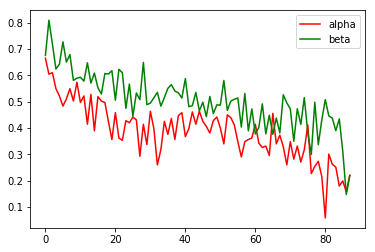
\includegraphics[width=0.6\linewidth]{../images/1b.png}.
\caption{$\alpha_i$ and $\beta_i$ are plotted.}
\label{fig:alpha_i_beta_i}
\end{figure}

\paragraph{c)} $u^{(1)}, u^{(2)}, v^{(1)}, v^{(2)}$ are computed as following. From the SVD on $Q_X^T Q_Y$ we can get different sets of singular vectors associated with different singular values, therefore we can get different $u, v$ through different sets of singular vectors. 
\begin{lstlisting}
	u = Qx@phi
	v = Qy@psi
\end{lstlisting}

\paragraph{c)} The largest singular value we get from SVD on $Q_X^T Q_Y$ is 0.66305211. The cosine of the angle between $u^{(1)}$ and $v^{(1)}$ is calculated using the following code, and the result is 0.65207818. They are very close to each other.
\begin{lstlisting}
	u[:, 0].T@v[:,0] / np.linalg.norm(u[:, 0])/ np.linalg.norm(v[:, 0])
\end{lstlisting}

\subsection*{Problem 2}
Data is loaded first using the following code. Data is also mean-centered. 
\begin{lstlisting}
	mat = spio.loadmat('data/MNFdata.mat', squeeze_me=True)
	X = mat['X']
	X = X - np.mean(X, axis=0)
	Xs = np.vstack((X[1:, :], X[0, :]))  # shifted X
	dX = X - Xs
\end{lstlisting}

\paragraph{a)-i)} The following code finds the maximum noise fraction basis $phi$ by solving the eigenvector problem. 
\begin{lstlisting}
	Y = np.linalg.inv(dX.T@dX/2)@X.T@X
	w, psi = np.linalg.eig(Y)
	phi = X@psi
\end{lstlisting}
The following code finds the maximum noise fraction basis $phi$ by solving the generalized eigenvector problem. 
\begin{lstlisting}
	import scipy
	C = X.T@X
	D = dX.T@dX/2
	w, psi = scipy.linalg.eig(C, D)
	phi = X@psi
\end{lstlisting}
The following code finds the maximum noise fraction basis $phi$ by solving the GSVD problem. Because python does not have a gsvd() function, I called the gsvd() from matlab in python.
\begin{lstlisting}
	import matlab.engine
	eng = matlab.engine.start_matlab()
	u,v,x,c,s = eng.gsvd(matlab.double((dX/np.sqrt(2)).tolist()), matlab.double(X.tolist()), 0,nargout=5)
	psi = np.linalg.inv(np.array(x).T)
	phi = X@psi
\end{lstlisting}

\paragraph{b)} The basis vectors from different methods are shown in figure~\ref{fig:basis_vectors_evec}, \ref{fig:basis_vectors_gen_evec} and \ref{fig:basis_vectors_gsvd}. All three methods seem to be able to separate noise and signal, and generate similar basis vectors. Some of the basis vectors have different direction, thus the figure seems flipped along x axis. 
\begin{figure}[h!]
\centering
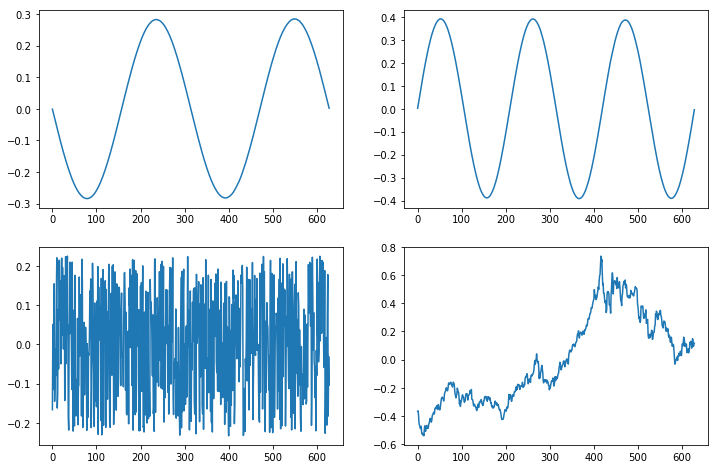
\includegraphics[width=\linewidth]{../images/2ai.png}.
\caption{Basis vectors from eigenvector method.}
\label{fig:basis_vectors_evec}
\end{figure}
\begin{figure}[h!]
\centering
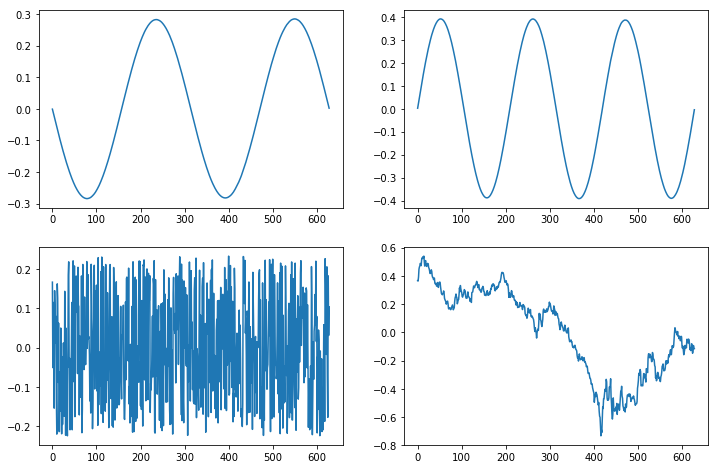
\includegraphics[width=\linewidth]{../images/2aii.png}.
\caption{Basis vectors from generalized eigenvector method.}
\label{fig:basis_vectors_gen_evec}
\end{figure}
\begin{figure}[h!]
\centering
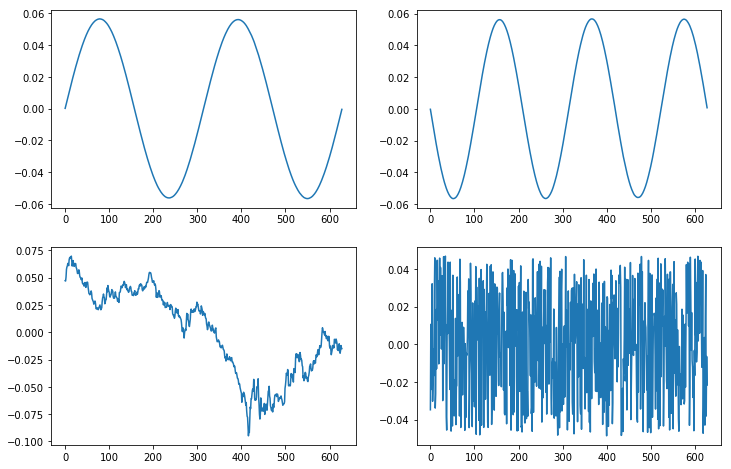
\includegraphics[width=\linewidth]{../images/2aiii.png}.
\caption{Basis vectors from GSVD method.}
\label{fig:basis_vectors_gsvd}
\end{figure}

\paragraph{c)} The following code is used to compute the SVD of the data matrix and plot the basis vectors. 
\begin{lstlisting}
	u, s, vh = np.linalg.svd(X, full_matrices=False)

	plt.figure(figsize=(12,8))
	for i in range(2):
	    for j in range(2):
	        plt.subplot(2,2, i*2 + j + 1)
	        plt.plot(u[:, i*2+j])
	plt.show()
\end{lstlisting}
Figure~\ref{fig:basis_vectors_svd} shows the basis vectors from SVD. SVD does not separate the noise with signal. This makes sense because SVD finds the best axis that maximizes the variance. 
\begin{figure}[h!]
\centering
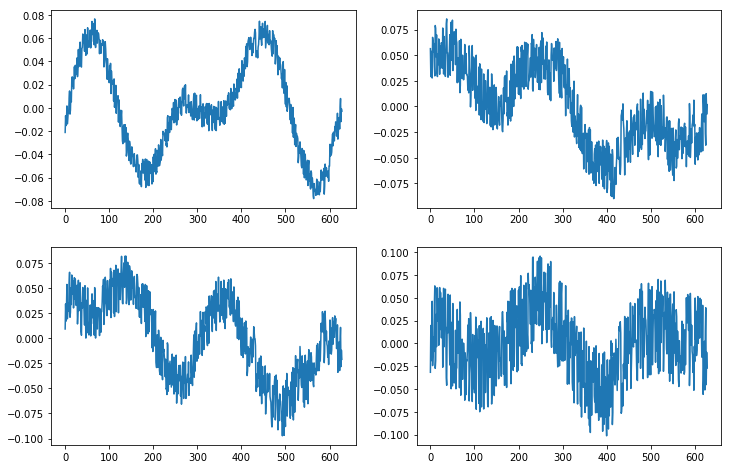
\includegraphics[width=\linewidth]{../images/2c.png}.
\caption{Basis vectors from SVD on data matrix.}
\label{fig:basis_vectors_svd}
\end{figure}

\paragraph{d)} The following code is used to project data matrix onto the first 2 MNF basis vectors and the first 2 SVD basis vectors. 
\begin{lstlisting}
	B_mnf = phi[:, :2]
	B_svd = u[:, :2]
	proj_mnf, proj_svd = B_mnf@B_mnf.T@X, B_svd@B_svd.T@X

	plt.figure(figsize=(12,8))
	for i in range(2):
	    for j in range(2):
	        plt.subplot(2,2, i*2 + j + 1)
	        plt.plot(proj_mnf[:, i*2+j])
	plt.show()

	plt.figure(figsize=(12,8))
	for i in range(2):
	    for j in range(2):
	        plt.subplot(2,2, i*2 + j + 1)
	        plt.plot(proj_svd[:, i*2+j])
	plt.show()
\end{lstlisting}
Figures \ref{fig:proj_mnf} and \ref{fig:proj_svd} show the projections. The projections on the MNF basis vectors are smooth because they are linear combination of two smooth curves. On the contrary, projections on the SVD basis vectors are noisy because the SVD basis vectors do not separate actual noise from signal. 
\begin{figure}[h!]
\centering
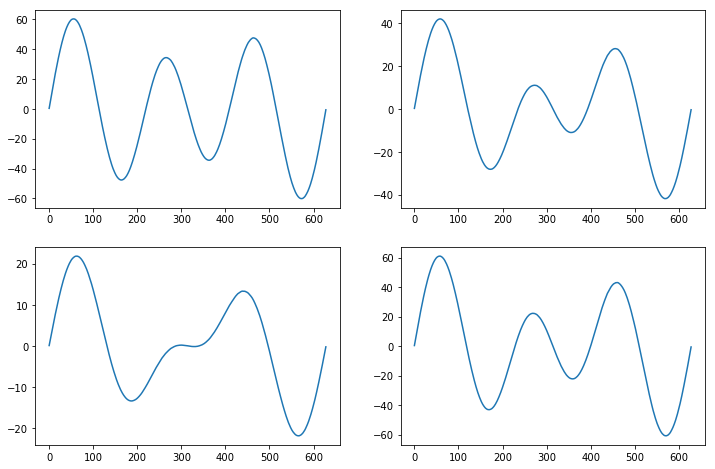
\includegraphics[width=\linewidth]{../images/2d1.png}.
\caption{Projection of X onto first 2 MNF basis vectors.}
\label{fig:proj_mnf}
\end{figure}
\begin{figure}[h!]
\centering
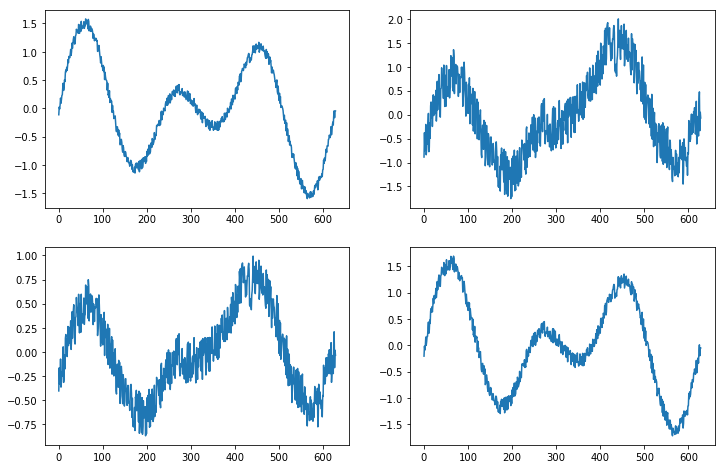
\includegraphics[width=\linewidth]{../images/2d2.png}.
\caption{Projection of X onto first 2 SVD basis vectors.}
\label{fig:proj_svd}
\end{figure}


\end{document}